\documentclass[a4paper,12pt]{report}
\author{Christian Bryan, Greg Opperman, Drew Wilson}
\date{\today}
\title{Broadcast Machine}

\usepackage{graphicx}
\usepackage{verbatim}
\usepackage{hyperref}

\begin{document}

\maketitle

% We need title page here. It has to be formatted as per the schools specs.

\chapter*{Abstract}
% One paragraph describing the project.

\chapter*{Authorship}
% Who wrote what.

\tableofcontents

\chapter{Introduction}
% A summary of the topics covered in this report.
% Describe the goal of the project.

\chapter{Background}
% FOR: Greg

\section{Introduction}
% Summary of the background section.

\section{Open-Source Software}
Open source software is an important part of the movement to democratize the media and Internet. 
This common goal is what ties together PCF's mission with that of the Free Software Movement. 
The goal of the Free Software Movement is to create software to increase the freedom of the public in general.\footnote{Richard Stallman, Why Software Should Be Free \url{http://www.gnu.org/philosophy/shouldbefree.html}}
Open-Source Software accomplishes this through its transparency, which inspires community development of software, and gives users the freedom to modify the software to suit their needs.
The software is Free in the sense that there are no conditions in distributing or using it, except that users respect the freedom of the software.

Without Free software, the Internet could not exist as a democratic medium.
Proprietary (meaning closed-source) software limits what users can or can't do with it, and does not give users the ability to modify code.
With proprietary software, users cannot \"own\" software, even if they purchase it.
Instead, users pay for the privilege of using it.
Under this model, the software is less accessible and less usable (as users cannot fix problems on their own, and must rely on proprietary developer support).
On top of this, other developers cannot learn from existing code, or base new work on it without paying costly licensing fees.\footnote{Ibid} 


Open-source software aims to build a cultural community of developers who can use each other as resources, learning from existing code, and freely building upon it to create new technologies altogether.
This culture encourages technological progress in ways that competitive, closed-source software does not. 

\section{The Current State of Internet Video}
As bandwidth and storage become increasingly cheaper, the prevalence of video on the internet has sharply risen over the past few years. 
In August 2006 alone, the number of people in the U.S who streamed video 
via the internet totaled over 110 million people, which is comparable 
with the number of households that watch traditional television.\footnote{http://paul.kedrosky.com/archives/2006/10/19/fun\_with\_intern.html}
The internet has allowed independent video producers a variety of platforms by which to publish and share their work. These platforms come in one of two forms: video hosting services, which offer a centralized location from which users can upload and share videos, and Content Management Systems (CMS), where users host and maintain their own collections of videos.

\subsection{Video Hosting Services}
Video hosting services are sites that offer free hosting and sharing of video files that users upload.
These sites, such as YouTube (\url{http://youtube.com}), Blip.tv (\url{http://blip.tv}), and Myspace Videos (\url{http://vids.myspace.com}) usually also offer social networking features, such as the ability to rate and comment on videos, as well as subscribe to videos posted by friends.
The largest and most popular video hosting service is Youtube, which garners 42.94\% of all traffic to online video sites.\footnote{\url{http://www.hitwise.com/press-center/hitwiseHS2004/videosearch.php}}. 

Video hosting services offer a convenient solution for video publishers 
to share videos with little technical expertise or resources, since bandwidth and hosting costs are shouldered by the service. These sites also allow users to embed videos into their own sites, giving them creative control over how the video is displayed. However, there are several limitations to this approach. In order to keep costs down and ensure that services remain possible under heavy traffic, most video hosting sites impose limitations that affect the quality of uploaded content. Having to service over 50,000 uploads a day, YouTube transcodes all of it's videos to a lower resolution, and imposes a limitation on the length of video clips \footnote{\url{http://www.youtube.com/t/fact\_sheet}}. 

None of the major video hosting services allow adult or objectionable content. Many sites regularly censor videos they deems inappropriate, including YouTube, who retains the right to control any and all content on its servers. Often, videos aimed at displaying legitimate discourse or expression are lost to this censorship\footnote{\url{http://www.nytimes.com/2006/10/09/technology/09link.html?ex=1318046400&en=e311caef3c3cf222&ei=5090&partner=rssuserland&emc=rss}}. For many publishers, the only way to ensure that their videos are presented correctly is to host them independently, using a content management system.

\subsection{Content Management Systems}

A Content Management System, or CMS, is a blanket term referring to the wide array of pre-packaged software used to manage website content. CMSes can encompass software to create wikis, forums, and several other collaborative mediums. In general, CMSes provide a simple user interface for adding, editing, and removing content, while obfuscating technical details. Using a CMS, it would be possible to build and manage an entire site without having knowledge of the underlying technologies and code. Most CMSes also offer robust theming engines, allowing users confortable with HTML and CSS to easily customize the look and feel of their site. Currently, the two most popular CMSes are Drupal and Wordpress.

\subsubsection{Drupal}
Drupal allows users to easily set up, create, and moderate blogs, forums, webpages, newsletters, and picture galleries\footnote{http://drupal.org/about}.
Written in PHP, it requires either MySQL v3.23.17 or PostgreSQL 7.2 or above\footnote{http://drupal.org/requirements}.
Thousands of popular sites use Drupal\footnote{http://DrupalSites.com}, including The Onion\footnote{ http://TheOnion.com}, OurMedia\footnote{http://www.ourmedia.org/}, and MTV's UK site\footnote{http://mtv.co.uk/}.

\subsection{Wordpress}
Wordpress one of the most popular weblogging applications, or a CMS designed specifically for posting text and image content by a small group of users.
Wordpress is PHP 4.2 and uses MySQL 3.23 as its database backend. 
It was created with the vision of creating a powerful GPL-licenced internet publishing platform based on open standards. 
The first version was released in 2001. 
Wordpress is blogging software designed to be installed on an individual's webhost, either their own computer connected to a broadband connection or a commercial webhost like Dreamhost or 1and1. There exist services such as the one at \url{http://Wordpress.com} that provide webhosting and just provide users with the a fresh install of Wordpress, but for the most part Wordpress users install the software themselves. 

Wordpress and Drupal both offer plugins for video publishing. However, there are currently no CMSes that directly address the needs of online video producers. There was a clear need for an easy to use, open-source, alternative to centralized video hosting service or complicated CMS plugins. With this in mind, the Participatory Culture Foundation (PCF), a Worcester-based non-profit, created Broadcast machine, an open-source video publishing platform.

\subsection {Broadcast Machine}
Broadcast machine is a content management system for video publishing designed to deliver videos via several different methods. Primarily, it acted as video blogging software, where users could organize videos into channels. Users could also subscribe to these channels using any RSS reader or desktop video software, such as Miro (\url{http://getmiro.com}. Broadcast Machine targeted users with little technological experience to offer a simple, easy-to-use user experience, and promoted alongside Miro (formerly Democracy Player) as part of a multi-tiered internet video platform, Broadcast Machine developed a strong following of users\footnote{A google search of the phrase \"Powered by Broadcast Machine\" returns approximately 6,700 results.}

Despite it's popularity, Broadcast Machine was plagued by a number of problems due to poor architectural decisions and sloppy programming practices\footnote{PCF's bug tracker reports 67 serious, unfixed bugs as of the time of this writing}. The original Broadcast Machine stored data in one of two ways: a MySQL database or a flat-file. However, model-layer logic was poorly abstracted from the rest of the application, and small differences between the two data-layer implementations caused several irreconciliable bugs. Since the program relied on a complicated and difficult to understand architecture, tracking down and fixing these problems became nearly impossible. Poor documentation, especially concerning Broadcast Machine's complex data structures, made it especially difficult for others developers to work on the project. Due to the aforementioned issues and lack of funding, development of Broadcast Machine was abandoned in 2006, to the dismay of its dedicated users.

\chapter{Design}

\section{Introduction}
Many of Broadcast Machine's current problems stem from its poor architectural implementation. 
To prevent these problems from happening in the future, Broadcast Machine must have a carefully-planned architecture that meets several design requirements.

\section{Ease of Use}
The most important requirement for Broadcast Machine is that it be easy to use. 
Broadcast Machine's target user, people who produce videos, should not need extensive technical knowledge in order to deploy and use the program. 
Just as a devlepor has almost no knowledge of how to shoot or edit a video, we should not expect the user to have any knowledge of PHP, RSS, or any of the technologies employed. 
Without being privy to any of the inner workings of the program, the user must be able to easily and intuitively publish videos and video channels via a simple administrative interface. 
Without any information besides their web server login and password, the user should be able to set up Broadcast Machine by dropping the application into their public HTML folder. 
The program should auto-configure itself on the first-run with a few simple clicks, even if the user is completely unaware of how his or her web server is set up. 
The application must detect server configurations that may interfere with its behavior, and handle those special cases gracefully. 
Likewise, viewers with any level of computer proficiency must be able to easily browse and download videos, leave comments and feedback, and subscribe to their favorite channels.

In order to ensure the best user experience possible, the new Broadcast Machine must be stable. In addition to this, it should preserve all of the functionality of its previous incarnation, while containing none of the unpredictable behavior.

\subsection{Customizable} 
A major feature of both the former Broadcast Machine and many other CMSes is the ability to customize the look and feel of a site running the software to fit the user's own personal style. 
As before, the application must be designed with a robust theming engine so that a user with only basic HTML and CSS knowledge can easily customize the website to suit his or her needs. 
Each users' site layout, or theme, will have the potential to look drastically different from each other with only minimal modifications to CSS and template code. 
The templates must be abstracted from the functional code, so that users need not worry about damaging the code or digging deep into its inner workings when modifying the layout. 
Users should also have the ability to easily switch between layouts. 


\subsection{Extensible} 
Similarly to the presentation logic, the application logic of Broadcase Machine must be structured so that it may be easily modified and maintained by any developer with relevant skills. 
The layout of the application should appear logical and concise, with a modular architecture to encourage programmers to freely add onto Broadcast Machine's feature set in order to meet their requirements.
The architecture should be transparent and have a well-documented API so that theses developers can start extending Broadcast Machine without exhaustive knowledge of the program, but merely a solid grasp of the documented data structures and class layouts. 
When features need to be added, the developers should be able to do so while maintaining the same architectural pattern and preserving the structure of the application, by adding only a few functions or classes. 
A well-structured, extensible architecture will prevent poor programming practices by encouraging developers to replicate the design patterns used to create the foundation of the application.


\subsection{Flexible}
In addition to additions to the program, Broadcast Machine must be flexible enough so that it can be re-factored easily. 
Functionality should be abstracted and delegated so that major changes to one part of the code will not affect another. 
For example, we may decide later that we would like to use a different type of database. 
We should be able to swap out the back end without having to modify the entire application, and without significantly affecting the user experience. 
In the event that bugs occur, localizing them to a specific section of code and implementing a fix should be possible without the fix appearing hacked together or thrown in. 
Developers should not need to dig through a mountain of code before finding the section that they need to edit. 


\subsection{Compatible}
The new Broadcast Machine must work across several different platforms. 
While impossible to guarantee compatibility with all web server configurations, Broadcast Machine most work on the most common web server setups. 
This includes any Apache web server with a minimal amount of installed modules, and most major hosting services (Dreamhost, 1And1, etc). 


\section{Features}
% This is just an outline right now. -Greg
There are several requirements for features that Broadcast Machine must include:
\begin{description}
\item[Automatic generation of RSS feeds]
\item[Templating system]
\item[Tagging]
\end{description}

\chapter{Implementation}

\section{Architecture and Languages}
Based on the aforementioned design requirements, it became clear that the program architecture needed to be modularized into three seperate parts. First, the presentation layer needed to be seperated from program logic in order to create a theming system by which users with basic HTML and CSS knowledge could customize the style of their site. In order to make the program both extensible and flexible for developers looking to add onto or modify existing Broadcast Machine code, it became necessary to further abstract data storage to be independent of both the presentation layer and the rest of the program architecture. This seperates the program into three layers, following the Model-View-Controller design pattern, or MVC\footnote{http://www.martinfowler.com/eaaDev/uiArchs.html}.


\begin{figure}[h]
\begin{center}
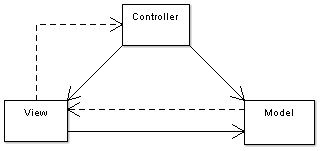
\includegraphics[scale=0.6]{./images/mvc.png}
\end{center}
\caption{Interaction between layers in MVC}
\end{figure}
In a pure Model-View-Controller architecture, all data is represented by the Model layer. The layer that the user interacts with, namely user-interface of the application, is represented in the View layer. The Controller layer represents the logic of the application, and in most cases, handles interactions between the Model and View layers. These interactions are shown in the figure above, with solid lines representing direct interactions, and dotted lines representing indirect interactions. Although in the general definition of this design pattern, the view can take user input and push it directly to the model, in most implementations it passes input to the controller for processing (input-validation), which in turn pushes the input to the model. Likewise, the view can also request data from the controller, who queries the Model layer. The query is then passed to the View for display and further user interaction.

There are several frameworks for implementing Model-View-Controller web applications, currently the most popular of which is Ruby on Rails. Ruby on Rails provides advanced features that allow automatic, rapid-prototyping of MVC applications, and object-relational mapping for controller interaction with the model layer, meaning that all data is automatically assigned to a class object based on the structure of the model layer.\footnote{http://rubyonrails.org} However, as a relatively new language, Ruby on Rails has not been widely adopted as other, more established languages. Very few basic web hosting plans support Ruby on Rails. To satisfy the requirement that Broadcast Machine be compatible with as many hosting and web server configurations as possible, we chose to write the application in PHP\footnote{http://php.net}. PHP is currently one of the most popular web scripting languages, and offers object-oriented programming features that allow for the development of a MVC application that adopts many of the design principles and features of a Rails framework. 

Similarly, MySQL is an open-source Database Management System (DBMS) that is perhaps the most widely used Structured Query Language (SQL) implementation, perhaps with the exception of enterprise-level applications such as Oracle. 
Like PHP, MySQL comes installed by default with most hosting plans, and setting up a database to be used with our application is a matter of running a script with the correct permissions. 


When choosing our DBMS, we must also predict how the application will scale with databases of varying sizes. 
An assumption that the average database will contain less than 1000 records for unique videos is reasonable. 
A publisher who produces a show daily would take almost three years to reach 1000 records, and most publishers release videos somewhat less frequently. 
Most of the queries on the database will be basic select statements for getting data, and insert or alter statements for adding or modifying video information. 
The predicted scale and function of our database would be best suited for a minimalist DBMS such as SQLite, which optimizes access to the data layer for smaller databases that do not need advanced functionality. 
Ideally, the program will be flexible enough to use SQLite when available, and require MySQL in all other instances. 
Architecting a flexible database controller will allow us to add other DBMS choices as necessary. 

\section{View}

\section{Controller}

\


\section{Changes to the Database}
In the new database model, several changes will have to be made in order to normalize the database for increased performance and easier programming. These changes are listed below:


The stats table has a one-to one relationship with the files table. This means that the two tables can be merged, and tracking the number of downloads can be relegated to a single field in the files table. The channel\_options table is also one-to-one with the channels table, so all of its data can be stored in the channels table.


The instance table can be replaced by a field in the channel settings for the base url of the website. We'll be able to assume that if, when a user goes to set up Broadcase Machine, the base URL has been filled already, then more than one copies of the program are sharing the database. Then, the user will be given a warning and a choice to overwrite this information with the new site.


A number of fields and tables will become deprecated in the new model. CSSUrl, from the channels table, will be replaced by the new templating system. As features associated with channel\_sections are widely unused, they will also be left out of the new schema, but may be added back in later. The files table contains the runtime of the video via three fields, RuntimeHours, RuntimeMinutes, and RuntimeSeconds. These fields will be combined into one runtime field representing the time in seconds, which will be converted into the h:mm:ss format in the file view rather than at the data-layer level.


The files table is poorly named, since it really stored information on videos, not the files that the videos are encoded in. In the future, it should be possible to have multiple files associated with one video (for hosting multiple formats and resolutions). The name of this table should be changed from files to something more descriptive, such as videos.


In the users table, the primary key field is Name, which may have caused problems when two people with the same name would attempt to register (e.g. two John Smiths would not be allowed to join at the same time). In the future, the primary key for the table should be username, which should always be unique.


Site settings will be moved from a B-Encoded file to a table in the database. Since we will be using http-seeding of torrents, some of these settings are expected to change.

\section{Architecture}
%This probably isn't too latex friendly yet - Greg
%^^ Jan/31/06: next time you want to use a list, use the item[] tag -drew
Active development began with discussions of how to best architect Broadcast Machine with a defined set of features:
\begin{description}
\item[Unit tests for all of the implemented functionality]
\item[A web based setup process]
\item[Creating channels]
\item[Browsing Channels]
\item[Managing channels]
\item[Creating video items from links]
\item[Creating video items from uploaded files]
\item[Browsing videos in a channel]
\item[Managing video items]
\item[Video RSS in all the forms curently available]
\item[Subscribe via Democracy link]
\item[User Authentication and permissions]
\item[Ability to import data from an existing Broadcast Machine]
\item[BitTorrent tracking]
\item[BitTorrent seeding via HTTP seeding support]
\end{description}


\subsection{Flow}
We then decided on a logical process for how the application would handle requests for information.
First, the application would receive a URL, POST parameters, and cookie information from the web server.
URLs will be typically received from mod\_rewrite in the form of http://baseurl.com/controller/action.
The action field may also reference another controler, in which case it would be followed by another parameter for the action that the controller should take.
For example, say a person runs a Broadcast Machine install on http://foobar.com.
If a user would like to browse all videos on the site by a specific category, such as \"dogs\", he or she would go to http://www.foobar.com/tags/dogs/.
In this case, \"/tags\" is a reference to the tag controller, which is responsible for getting all videos that contain that tag.
The parameter to be passed to the video controller is \"dogs\", which means that only videos containing the dogs tag will be returned.


After the controller generates an associated array of data (which may contain other arrays), it passes this information to the view layer, or the template.
The template uses this information to fill in an XHTML or RSS page, and sets the mime type (in the case of linking to files), and renders the user interface.


\section{Program API}
Next, we considered the program API, or the way in which the actual code and data would be laid out.
This affects not only the program itself, but also how developers would go about adding new features and modifying existing ones.


\section{Controllers and Views}
After coming up with an acceptable API, our next task was to come up with a list of views, and delegate responsibilities for getting the data necessary to render those views to the appropriate controller.


\subsection{Front Page (/)}
The front page is found at the top directory of the Broadcast Machine install (\"/\").
This page lists all of the viewable channels.
If a user is logged in as an administrator, it also provides links to add, edit, or remove that channel, as well as subscribe links for Democracy Player, RSS, and iTunes (depending on the site settings).
The controller responsible for getting the information about each channel is aptly named the frontpage controller.


\subsection{Channel View (/channelname)}
The channel view lists all videos in a channel, and is accessed by going to a URL-safe truncation of that channel's name.
This view calls the channel controller to retrieve information about every video in the channel, and then inserts that information into the template.
The view also displays channel statistics and subscription links.
If you are logged in as an administrator, there will be buttons to edit, delete, or add new videos, which each correspond to appropriate video controller actions.
Administrators also have the ability to see links to delete the entire channel, or edit it.


Adding a video to a channel is handled by the \"add\" action of the channel controller (\"/channelname/add\").
When adding a video, users will be able to enter detailed metadata about the video, and either link directly to the file or upload it directly to the server, albeit with restrictions\footnote{PHP has a maximum file size for uploading that depends on the server configuration}.
Users will also be given the option to upload the file on their own via FTP, and have Broadcast Machine detect it later.
Similar to adding videos, there will also be appropriate channel controller actions for removing the channel (\"/channelname/remove\") and editing it (\"/channel/edit\").


\subsection{Video View (/video/videoname) }
The video view displays all of the relevant information about an individual video, including its meta-data and download statistics.
It will optionally display a video preview of the file instead of a static thumbnail image. The view will also generate a link to download the entire file.

\subsection{Tag View}

\subsection{User Administration (/users) }
The user

\section{Model Schema}

\section{Testing}

\subsection{Unit Testing}

\subsection{User Testing}
% 2/8/2005, CJ: Wrote about the use of unit testing, its advantages and the setup of the test servers.
With any software, it is necessary to test to make sure that your application works as expected.
We decided to test our application on mock servers so that we could see how our software reacted to common configurations that we expect our users to encounter.

We ended up with three server configurations:
\begin{description}
	\item{Generic Linux} This server runs a common version of Linux called Ubuntu. It is running Apache 2 as its webserver with PHP version 5 and both MySQL and SQLite databases. This configuration is optimal, and we feel that it will account for the majority of our users. It is also important to have support for both database engines; we need to make sure that the program behaves correctly when both are available.
	\item{Microsoft Vista} Having a server that is running Microsoft's Internet Information Services is important. 
Because IIS is the second most popular webserver in use, we need to make sure that we are not preventing such a large population from running our software. Ensuring that our application runs on IIS will be difficult because of it's lack of URL rewriting support. It's important to us that our program run on servers lacking URL rewriting, because while it is convenient and common, its availability cannot be guaranteed. Fortunately that will be the only challenge on this server; its configuration is otherwise similar, sporting PHP 5 and SQLite.
	\item{Hosted Linux} Since our program is geared towards users who are likely to have low-cost hosting services, we decided to use one popular service as a testbed. Dreamhost provides inexpensive, albeit limited hosting accounts. They provide servers with Apache 2, PHP 4, and MySQL installed. The platform provides us with a place where we can see how our program deals with setting permissions in restricted environments.
\end{description}

These testing platforms should do a good job at allowing us to see how our application is coming along.
It lets us see how the smaller pieces work together, but it does not let us see how the smaller pieces are working by themselves.
If the smaller parts do not work then the whole will fail.
This is the point where unit testing becomes useful.
Unit testing allows our group to write small pieces of code that test individual classes and functions.
When we see something go wrong on the testing server we can run our unit tests and pinpoint the part of the program that we need to fix.
Between the use of the testing servers and the unit tests the goal is to minimize the amount of time that we spend diagnosing bugs and instead spend more time fixing bugs.

Overall I feel that these servers will be as useful as we expect.
They will help us be as prepared as possible when it comes time to release the first version.
This testing framework should also be very helpful to anyone who would like to continue developing Broadcast Machine.
The unit tests will make sure that the existing code does not break, and the test servers illustrate what our target environment is.
Unfortunately it took a very long time to get the test servers running.
The amount of effort put in to setting up the testing framework seemed excessive to me.
For a project of this size, I can't say whether or not the time spend was worth it.
Hopefully these are useful to future developers and our time was well spent. 

\chapter{System in Action}
% FOR: CJ

\chapter{Results}
% FOR: Greg

\section{Unit testing}

\chapter{Feedback}

\section{Mike Benedetti}

On February 23, 2008 we met with Mike Benedetti, the webmaster from Worcester's Community Cable Access (WCCA) Channel 
13. 
Benedetti used our software and made comments on it as he navigated the interface. 
Our major goal was to determine if his expectations for the interface meshed well with where our software was heading. 
Through our discussion with him we discovered is even more a part of the internet video community than we had expected. 
As a result he was able to also offers insight into where our software fit into the landscape of internet video.

WCCA has recently begun putting all of their video content online. 
They currently use Drupal with a number of modules as their content management system, but Benedetti explained to us 
that there were a number of drawbacks with his current setup. 
Through our research we have come to many of the same conclusions as him, but it was valuable to hear frustrations about 
other software solutions from someone with first-hand experience. 
Mike stressed that there was not yet a one-stop video content management system, although he did point out that there 
exist plugins and modules for existing CMS's that transforms them into a make-shift video CMS. 
He indicated that dispite a number of solutions, there was a need for a .wordpress for video..

We started our discussion by having Mike outline the procedure that WCCA follows to move video content from a recording 
studio to the web. 
It is the following: 

\begin{enumerate}
\item A content producer records a show in their studio. 
\item The show is edited and cut down to fit the time-slot.
\item The show is aired on the cable station. 
\item Mike uploads a high-quality copy of the video is to archive.org. He must input various attributes of the video, 
including the title, text description, director, producer, production company, keywords and information about the audio 
and visuals. 
\item Archive.org's servers then convert the video into a number of file sizes and formats and make the files publicly 
available.
\item Mike embeds a lower-quality version of the file in a post using Drupal. Mike must re-enter all of the video 
attributes at this point.
\item The video is posted to the WCCA site and Drupal handles adding an entry to the video rss file.
\end{enumerate}

After we talked with Mike about his setup, we opened up a browser and had him explore our software. At this point we 
asked him to follow links and describe what his exceptions for the pages were and compare his expectations to the 
reality of our pages. 
It was valuable to hear that Benedetti's expectations for the views were somewhat different than what we had. 
There were a few specific UI suggestions that he had, but most important suggestion was molding our visual design on the 
concept of a .river of news.. 
He explained that it made more sense to him to have the videos appear in a more traditional blog layout, with clear 
differentiate between .posts. and with a publish date clearly indicated. 
He also pointed out that we needed to make it clear that the rss feeds were video rss feeds that could be used with 
programs like Miro.

He gave further feedback on the rss feeds. 
Specifically, he did not see much value in the non-video RSS feeds--for example, a feed of all the tags or of all the 
channels. 
We discovered that it needed to be made more clear that the video feeds had enclosures. 
The issue may be resolved by simply moving the RSS icons to a better location.

More broadly Benedetti gave us a feel for where broadcast machine fits into the landscape of internet video. 
He seemed to be hopeful about our project and it might be a good fit for his needs.
He is of the opinion that there still does not exist a solid one-stop solution for a video blog. 

As was mentioned ealier, WCCA uses archive.org as their long-term storage. 
Mike suggested that Broadcast Machine would be a more appealing piece of software if, in a future release, it 
incorporated an easy mechanism for external storage solutions. 
We looked at WCCA's account and found that there is an XML API provided for archive.org to integrate with external 
software. 

Meeting with Mike Benedetti gave us a good perspective on how users would see our software. 
We did not incorporate all of his suggestions, but we did make a number of good changes based on his ideas. 
It was encouraging to hear that the software that we created could be used by as large as organization as WCCA.

\section{Specific Suggestions for Improvement and Our Responses}

\subsection{Suggestion: "River of news"}

Mike Benedetti found that our UI was not exactly what he was expecting. 
He offered the design concept called the .river of news., and recommended that we use it in our user interface. 
"River of news", as he explained it, is the idea that there is a visible flow of information, that each post is clearly 
shown as an incremental addition to the site. 
He suggested dividing video posts more clearly, making the video title more of the focus of the post, and including a 
post date or timestamp in a more prominent location. 
When I asked if he felt there was not enough meta-data provided about a video, he replied that there was enough data but 
that it should be more clearly divided and laid out. 

\subsection{Our Response}

Mike's suggestion "river of news" idea resonated well with us. 
Our software is a video blogging platform, so it makes sense to model our design after traditional blog themes. 
Although, it is important to note that almost all of Benedetti's design suggestions can be changed by an end-user with 
some HTML knowledge. 
This shows the versatility of our templating engine. 
Someone who intalls Broadcast Machine can just open up the smarty files and layout and style the pages however he or she 
feels appropriate. 
However, Mike is right that a "news river" design makes sense as the a sane default for the software. 
It will better fill the needs of average user. 

As a result, we incorporated some changes. We updated the video/all page. 
We brought the title above the icon and made it more prominent. 
Then we moved the modified\_time timestamp to directly below the video 
title to give some sense of continuity. 
We added a larger area for the video description, changing the truncated length from 100 characters to 350. 
We moved the metadata to the left of the icon to save space and moved the description to below the icon. 
Then we added a divider at the end of the video post. 

\subsection{Suggestion: Remain consistent about video/channel order}

There are a number of pages that list both channel and video data. 
Namely, Mike noticed that on the channel/all view and the tag/all view we were not consistent about which came first. 

\subsection{Our Response}

We went through the views and made sure channel data was always place above video data.


\subsection{Suggestion: Make it more clear what data is in the rss feeds}

Benedetti indicated that he was confused about what data was in the rss feeds, based on their placement. 
The icons are just a standard rss icon, so also they did not offer any clues. 

\subsection{Our Response}

After reviewing the placement and icon images for the rss links, we decided to take two actions.
We moved the rss icons to a location on the page that more clearly indicated their content. 
For example on the tag/example-tag view, the rss icon was previously placed next to the header that read, .Items tagged 
with 'example-tag'.. 
This was confusing because we had both channel and video data displayed on the page. 
Since the rss was a video feed with only metadata and enclosures from videos that were tagged with the given tag, it was 
misleading to place the icon at the top of the page. 
We removed the rss icon from the header and added one next to the sub-heading for videos. 

Secondly, we added a second rss icon from the Miro website. 
It reads .Miro Channel. and provides a subscribe-in-Miro link. 
This should make it more clear that the feed is a video feed, which can be added to a video rss reader. 

\subsection{Suggestion: Bit torrent support}

Mike recalled that the previous version of Broadcast Machine was based on Blog Torrent, which meant that support for 
BitTorrent was once included. 
However, he also recalled that he never got BitTorrent working properly when he used the earlier version of Broadcast 
Machine.this is an experience shared with many other early Broadcast Machine users. 
He thought that BitTorrent support would be a good addition.

\subsection{Our response}

The project has changed dramatically since its inception. 
BitTorrent support was originally part of our plan for Broadcast Machine. 
Since other aspects of the project ended up taking more time than we had originally expected and since BitTorrent 
support turned out to be a larger issue than we had anticipated, we had to drop its support for this version on the 
software. 
We agree with Mike that it is a very good addition. 
We hope it will be in a future version.

\subsection{Suggestion: Integrated external hosting}

Since WCCA cannot afford the bandwidth to host all of their own video, they store their video remotely in their 
archive.org account. 
Mike thought it would be ideal if Broadcast Machine could easily integrate with archive.org, amazon s3 or other third 
party hosting services. 

\subsection{Our response}

We are very fond of Mike's idea and believe it would be very useful for some of our users, but we decided against 
incorporating his suggestion. 
There are a few reasons why. 
Most importantly is an issue of time. 
An addition like that would take a significant amount of time to build. 
We simply do not have enough time before the end of the project to incorporate the new functionality. 
We have determined that it is a good enough idea that it may be incorporated in a later version. 
However, there is also the issue of maintaining the code. 
There is an ever-changing number of third party hosting services. 
Maintaining support for them be a substantial undertaking. 
It would most likely require a person or group of people who are passionate about the functionality to keep it working 
with the external hosting solutions. 
Although we decided against incorporating the change, we believe we have built a framework that is extensible enough to 
allow an enthusiastic programmer or group of programmers to add that functionality to Broadcast Machine themselves.

\chapter{Future Work}
% FOR: CJ
% Talk about how the package will be maintained as an open source project.
% Features that should be added: BitTorrent, Flash Video, Advanced (AJAX) UI,
% Flash-based uploader, Internationalization, 


\chapter{Conclusion}

\appendix
\chapter{Former Broadcast Machine Documentation}

\section{Data Model}


\subsection{Instances}
The instance table was used to prevent two versions of Broadcast Machine from using the same database. In the previous version of Broadcast Machine, if more than one site was using the same database, a warning was displayed on the main page of the administrative interface. The table consists of a hash string of the hostname (id), and a timestamp for when the instance was created (time). 


\subsection{Stats}
The stats table allowed the user to keep track of the number of user downloads for each video. It contained a unique hash of the filename (id), and an integer for the number of downloads (downloads). The table has a one-to-one relationship with files.


\subsection{Channels}
The channels table was used to store metadata about specific RSS video feeds, or channels. This data was used to generate the channel view and RSS feeds for each channel, which is how most users interact with the application. 
%Show a screenshot of the channel view, perhaps?
It contained a unique integer identifier (ID, the primary key), A text explanation of the channel (description), and integer number for when the channel was made (Created), a text title for the channel (name), fields for URLs of linked icons, libraries, and the channel's main website (Icon, LibraryURL, and WebURL, respectively), a field to designate the publisher (Publisher). In addition to this, it has several tiny int values that served as settings flags, with 0 being false, and the default value, and 1 being true. This includes OpenPublish, RequireLogin, and NotPublic. OpenPublish allowed administrators to designate whether or not non-administrative users were allowed to publish videos to a channel. RequireLogin was used to determine whether or not users must be logged in to view the channel. If NotPublic was set, the channel itself would be hidden from anonymous users.
It also contained CSSURL, which would store a link to an external style sheet to be used in rendering the channel page.


The channel\_options table keeps track of the individual settings for a given channel. Each record in the table contains an integer reference to the channel it refers to (ID). Several boolean flags determined which information about a video would be shown on the channel view: Creator, Description, Filesize, Keywords, Length, Published, Thumbnail, Title, Torrent, URL. There is also a tiny int field called SubscribeOptions, whose default value is 7. This value determines which subscription links will be made available to users (RSS, Democracy, and iTunes, which requires direct URLs to be enabled in the site settings). In this field, RSS is represented by a value of 1, Democracy by a value of 2, and iTunes by a value of 4. Adding together the values of available subscription links determines the field's value. For example, A value of 7 means that all links are available for use, while a value of 1 would mean that only RSS could be used. A value of 6 would mean that iTunes and Democracy subscription links should be made available. 


The channel\_files table records associations between the channels table and the files table (see below). In other words, it allows Broadcast Machine to keep track of which files belong to which channel, which is essential to the channel view and RSS feeds. It contains a reference to the channel in question (channel\_id), the hash of the file (hash), and integer timestamp (thetime). The primary key is channel\_id and hash, meaning that there can't be more than one record for any channel and file pair.


The channel\_sections table allows channels to be split up into several subsections. From experience, this seems to be widely unused by BM's user base, and is also not implemented in the RSS view. As such, it may be deprecated. The table itself contains an integer reference to the channel the record refers to (channel\_id) and the name of the section (Name). The table also shares a one-to-one relationship with the channels table.


Like channel\_files, the section\_files table tracks which files are associated with which sections. The table contains a reference to channel\_id, a reference to the name of the section, and the hash of the file. The combination of those three fields are a primary key and must be unique.


\subsection{Videos}
The table for storing video information is the files table. This information is used to render the details page for each individual video. The files table contains a unique integer identifier for each video (ID), an ineger for when the file was created (Created), the name of the file (FileName), the name of the person who created the channel (Creator), a text summary of the file (Description), a title (Title), an optional link to a transcript for the hearing-disabled (transcript), a link to a website for more information(Webpage), an optional donation code (donation\_id), boolean flags for Excerpt, Explicit, ignore\_mimetype, and External properties, and URL, in case the file was linked to externally. It also contains a link to an image thumnail of the video (Image), name and URL of the license used to distribute the video (LicenseName, LicenseURL), the MIME-type of the file (Mimetype), an integer for the date published (Publishdate), and the date of the video release via three fields: ReleaseDay, ReleaseMonth, and ReleaseYear (all are integers). Also included is a short string called Rights, which is slightly redundant due to the License field. 


Records of people who have contributed to the making of a video were stored in the file\_people table. This allowed administrators to include conprehensive credits for anyone working on the video. The table contained an identifier for which video the credit refers to (ID), their name (name), and what they were credited for (role). The combination of these three values were required to be unique as a primary key.


\"Tags\", or categories to classify videos by, were stored in the file\_keywords table. This allowed administrators to classify videos by category, so that users could browse videos in that category across many channels. This table contained an ID reference to the video, and then the keyword that the video would be tagged by. Although one video may have had many tags, no video could have two identical tags.


\subsection{Donations}
The donation table stores information on how users can contribute to the makers of a video. This allowed the generation of donation links to be displayed alongside a video in the video view, as well as from within Democracy and the RSS feed for the channel. Users could use these links to contribute to the makers of the video. Each donation record had a unique ID, an e-mail address (email), a short description (title), and a longer text donation pitch (text). Putting this information in its own table allowed publishers to frequently associate videos with the same donation info, as this info rarely changed. 


The donation\_files table links together donation info with video info. The table conatined the id of the donation info, as well as the hash id of the video (hash). Each video could only be linked to one set of donation information, so id and hash are both primary keys.


\subsection{Users}
The user table contained information about registered users. This table contained an alias for each user (Username), the user's real name (Name), their encrypted password (Hash), their e-mail address (Email), when they registered (Created), and their permissions information (IsAdmin, IsPending). 


The newusers table tracked only those users who have not verified their account. This allowed functionality to prevent scripted bots to spam Broadcast Machine installations with open registration, by requiring that all users verify their e-mail address. The table included a filehash, their password (Hash), their e- mail address (email), IsAdmin, and when they created the account (Created).


\subsection{Settings}
Settings for the website itself was stored in a B-Encoded flat file. This allowed users to customize site security features, as well as which features they wanted to use. This is also where essential information such as database connection settings were stored. These fields include whether or not new user registration was allowed (AllowRegistration), whether or not they required approval (RequireRegApproval), whether or not they needed to verify their account (RequireRegAuth), whether or not users could upload or download anonymously (UploadRegRequired and DownloadRegRequired, respectively), the default channel (DefaultChannel), whether the site has channels that anyone could modify (HasOpenChannels), their current site layout (theme), title of the site, the site description, an image associated with the site, the base url for the site (baseurl), database connection settings (mysql\_prefix, mysql\_host, mysql\_username, mysql\_password, mysql\_database, and mysql\_verified), and BitTorrent sharing settings (Ping, sharing\_enable, sharing\_auto, sharing\_python, sharing\_actual\_python, minport, maxport).

\chapter{Disorganized Mess}
\section{New Model}
%This will be changed and updated as the new schema comes along further
%Needs: People should be relational!
Broadcast Machine must keep track of several pieces of information pertaining to its entities (channels, files, etc.).
A comprehensive list of the data follows (entity relationships highlighted in bold):


\subsection{Data associated with Channels}
\begin{description}
\item[Channel ID] An arbitrary, unique number to identify the channel and  associate it with other entities
\item[Title] Each Channel has a title, represented by a string
\item[Description] A longer body of text that describes the channel's theme or content
\item[Icon] Reference to the thumbnail image (See below)
\item[Credits] A list of the channel creators and maintainers, or any other people involved.
\item[Donation information] Represented as a snippet of HTML or a simple url.
\item[Website information] A url to link to the channel's main web page.
\item[Tags] 0 or more keywords associated with the channel, used for categorizing and browsing multiple channels.
\item[Permissions] Rules about which users can access or modify the channel
\end{description}

\subsection{Data associated with channel tags}
\begin{description}
\item[Video ID] A reference to the video that the tag describes
\item[Tag name] A short word or phrase to categorize the channel
\end{description}

\subsection{Data associated with Users}
\begin{description}
\item[ID] An arbitrary, unique number to identify the user and associate him/her with other entities
\item[Username] The user's nickname or handle
\item[Password] Self-explanatory
\item[Email Address] Optionally used to verify registration
\item[Permissions] User's access credentials for specific channels, files, and the site in general
\end{description}

\subsection{Data associated with Videos}
\begin{description}
\item[ID] An arbitrary, unique number to identify the user and associate it with other entities
\item[Title] A short amount of text to describe the video
\item[Description] A longer body of text that describes the video's theme or content
\item[Last Modified Date] A time stamp set every time any video information is changed.
\item[Credits] A list of the channel creators and maintainers, or any other people involved.
\item[Icon] Reference to the thumbnail image (See below)
\item[Transcript (optional)] A text-version of the video's content or dialog for the hearing impaired
\item[License/Copyright information] The name of the license associated with the content, and possibly a url to link to the full body of the license
\item[Website url] A link to the video  or publisher's website
\item[Release Date] The date and time the video was released to the public
\item[Publish Date] A timestamp of when the video is made available to the public. note that this is different than release time (For example, a publisher might publish a movie that was released at an earlier time elsewhere).
\item[Running time] The length of the video, in seconds
\item[Adult] A boolean flag used for marking adult content
\item[Donation information] Represented as a snippet of HTML or a simple url.
\item[Tags] 0 or more keywords associated with the channel, used for categorizing and     browsing multiple channels.
\item[Mime-type] The type of media that the file represents
\item[Filename] the url or address on the server where the file is located
\item[Size] the size of the file, in bytes.
\item[Downloads] A running count of the number of users who have downloaded the file
\item[BitTorrent Information (optional)] If the file is a torrent, additional information must be stored (see below)
\item[Permissions] Rules about which users can access or modify the video
\end{description}

\subsection{Data associated with video tags:}
\begin{description}
\item[Video ID] A reference to the video that the tag describes
\item[Tag name] A short word or phrase to categorize the video
\end{description}

\subsection{Data associated with icons}
\begin{description}
\item[Icon ID] A unique, autogenerated id number to identify the image
\item[Icon URL] The address of the icon
\item[Mime-Type] The type of file that the icon is
\end{description}

\subsection{Design Decisions}
The current schema departs from the previous data structures in many ways.
Previously, the data layer was represented as a flat-file database.
Although most of the data structures were organized in a normalized, logical way, there were several inconsistencies that needed to be reconciled.


First, several pieces of data were being improperly stored in the database. 
For example, channel and site settings were being stored in the database. 
This information doesn't typically belong in a relational data structure, simply because it does not interact with other entities, nor can it benefit from any of the features of a database. 
Instead, we decided that the data belongs in a simple, transparent configuration file as part of the template system. 
That way, data can be easily read and modified, both by the application and advanced users. 


Channel icons and video icons, are no longer exclusive, and have been combined into a single icon table.
This means that the same icon information can be used by both channels and videos. This will help eliminate duplicate data, and give users more choice in choosing icons.


The new schema also drops several fields and data structures that could be simplified or generated on the fly.
For example, in the previous version, thumbnails were represented as their own entities, because the database stored the mime-type as well as the file address.
Since most, if not all, browsers render images without an explicit mime-type, eliminating this field also allows us to simplify the schema by storing all of the thumbnail information in the channels and video tables themselves.
Similarly, fields like file extension, which can be derived from other data, have been pruned.
We also store information about intellectual property licenses that could be abstracted to its own table.
However, this doesn't provide any significant functional benefits, so the information has been moved to data fields in other tables. 
File data and video data have a one-to-one relationship, so it makes sense to merge them into one table.
This will normalize the table, which will optimize queries and simplify queries that access that data.


%% Move to design
\chapter{Utilized Technologies}
\section{Apache}
% 1/18/2007, CJ: Rewrote it to be more concise.
We chose the Apache webserver as our target environment because of its prevalence among low-cost web hosts.
Because the audience we are trying to reach is likely to be running on a tight budget, we are making the assumption that they will choose a low-cost host.
Even outside of this class of service providers, Apache retains market share dominance; so even when users might want to move to a better hosting solution Apache is right there with them. \footnote{From a Netcraft survey spanning Oct. 1995 through Jan. 2007. http://news.netcraft.com/archives/2007/01/05/january\_2007\_web\_server\_survey.html}
Another advantage is that it is very common for PHP and Apache to be installed alongside one another.
With the popularity of the \"L.A.M.P.\" server configuration it is reasonable to make such an assumption.
Apache's support for per-directory configurations via an .htaccess file make it very easy for users and developers to customize the environment without specialized administrator access.
These in-directory configuration files also do not require costly server restarts.
As for Microsoft's IIS webserver, we will make sure that our program runs on the server, but there will be no guarantees that it will be particularly elegant.


\section{PHP}
% 1/18/2007, CJ: Rewrote to be more concise. Perhaps talk about PHP vs. Perl, Python, Ruby
Our team chose to write this application in PHP because it is the one server-side scripting language that is guaranteed to be installed virtually everywhere.
As noted previously, it is often installed alongside Apache and there are many service providers that already have it installed on their servers.
PHP as a language is dynamic and weakly typed with a C-like syntax and a large standard library set that geared towards web development.
Other languages such as Perl, Python, or Ruby might be excellent choices, but they do not command the same percentage of the market share that PHP does.


\subsection{Cookies/Sessions}
% 1/19/2007, CJ: Added part about user authentication.
Web applications almost always require users to be authenticated and tracked in some way, and PHP provides convenient ways to do both.
Classic username/password authentication can be used to quickly verify the users identity and through the user of built in session\_* functions in PHP we can easily create persistent user sessions.
More details on how this functionality will be used can be found in the implementation section.


\section{SQL}
% 1/18/2007, CJ: Nassar suggested that there should be some mention of object vs. relational databases here. I don't think there's much to talk about!
To store all of the information about the channels, videos and settings in Broadcast Machine, we decided that a relational database would be best. 
As opposed to previous releases, this version will only have SQL database support.
We figure that since the last release SQL databases have become commonplace.
PHP itself is proof of this, as it easily interfaces with MySQL and SQLite.
We feel that a database lets us store and retrieve data in the most scalable and efficient way possible without sacrificing the overall goals of the program.
It is important to note that the database setup will be automated for the user like it is with weblog package WordPress.
This automation helps us work around the problem of the user having to configure a complex database. (A great concern for us! Many of our users might not be very computer savvy.)


\section{URL Rewriting}
% 1/22/2007, CJ: Rewrote the section about URL rewriting.
In the past few years, URL's have become more and more difficult to understand as web applications have come to dominate.
URL's were designed to be easier to remember than IP addresses, but the've shown they can be just as tough to remember.
One way to make URL's easy to remember is to rewrite them through the use of the Apache module mod\_rewrite.
This module rewrites making the server pretend that a file exists.
When it receives a request for a URL it modifies it based on pre-determined rules that can be set by the user.
These settings can be configured on a per-directory basis by placing the rewrite rules in the .htaccess file.
URL rewriting also serves another purpose.
Apple's iTunes will 
This feature is also necessary to make sure that iTunes can subscribe to feeds produced by Broadcast Machine.
iTunes requires that the file to be downloaded ends as a file extension that it likes.
Unfortunately those file extensions are not usually webpages, they are usually MP3 instead of PHP.
It will only download your MP3 if it looks like \url{http://www.foobar.com/index.mp3?show=4.mp3} versus the traditional \url{http://www.foobar.com/index.mp3?show=4.mp3}. \footnote{http://www.apple.com/itunes/store/podcaststechspecs.html}
Not convenient, but necessary given the popularity of iTunes and the demand for compatible content.


\section{XML and RSS}
% 2/2/2007, CJ: Finished the section. Needs a review/read-through and probably some corrections.
XML itself is a multi-purpose markup language specified by the W3C that provides an enormous amount of flexibility.
It's loosely defined syntax makes it suitable for almost any application imaginable.
One of the most prevalent applications of XML is RSS.
Lately the RSS specification has gained alot of traction as a useful and feasible format for distributing syndicated content.

The format was created as a way for publishers to distribute their content in a 
Unfortunately RSS has has a tumultuous past, with three different and competing versions the format was hardly standard.
The past few years have allowed RSS to mature into the document format that it is now.

XML, or Extensible Markup Language, is a general-purpose language for describing hierarchal relationships with a variety of applications. 
First recommended by the W3C in 1998, XML provides an easy way to convey information that is both human-legible and easily parsed by computer algorithms. 
XML documents start out with a declaration stating what version of XML is being used, information about character encoding, and any other dependencies that the document may rely on:

XML documents start out with a declaration stating what version of SML is being used, information about character encoding, and any other dependencies that the document may rely on:

<?xml version=\"1.1\" encoding=\"UTF-8\"?>

This tag specifies that the document is using the XML 1.1 standard, and is encoded using the UTF-8 character set.

Followed by the declaration, XML files consist of several elements that may be nested within each other, defined by start and end tags.
These tags surround text or other elements, which is referred to as the tag's content.
Tags may have attributes which are embedded into the element's start tag. 
The meanings of each tag and its corresponding content is left intentionally ambiguous, meaning that the XML standard allows users to define what signifigance the tags have, and what data they should contain. 
Customizable schemas supplement the syntactical rules of XML with constraints having to do with element and attribute names, and how the information is organized heirarchically. 
For example, a schema might specify that an XML document describing a bicycle must have an element describing the gears, and only one gearset must be present for a car. 
It might also specify that a set of gears can have several attributes, including manufacturer, number of gears, etc. 


<bike name=\"C200\"\ manufacturer=\"Raleigh\">

<gears manufacturer=\"Shimano\"\ speed=\"21\">Y-42U98010</gear>

...

</bike>


XML is a powerful markup language, and it has been used to construct many popular languages, such as XHTML and RSS.
RSS is an integral part of Broadcast Machine.
The format was developed to allow content producers to publish their content in a way that was easily syndicatable, standardized and inexpensive.
RSS went through an unfortunate period where many individuals and groups wanted undue control over what the standard was going to be.
Lately publishers have begun to settle on the RSS 2.0 specification.
While RSS 2.0 is not governed by a traditional standards body such as 
the W3C or ISO the specification is taken care of by the RSS-DEV working 
group at Harvard University. \footnote{\url{http://en.wikipedia.org/wiki/RSS-DEV\_Working\_Group}}
The RSS 2.0 specification allows for publishers to specify \'channels\' in which there are repeating elements of \'items\' which contain the main content.
At the top of the RSS file there is an area where the publisher can add information about the channel such as a link to the publishing website, the author, webmaster and other various information.
Each of the items within the channel contain additional sub-elements that describe the item.
There are descriptors for the time and date at which the content was published, links to the website with the extended or full version of the contents, and ususally there is a unique identifier that lets the computer detect duplicates. 

<?xml version=\"1.0\"?>
<rss version=\"2.0\">
  <channel>
    <title>Boston Concerts</title>
    <link>http://bostonmusic.org</link>
    <description>A collection of concerts in Boston.</description>
    <language>en-us</language>
    <pubDate>Tue, 10 Jan 2006 04:00:00 GMT</pubDate>
    <lastBuildDate>Tue, 10 Jan 2006 09:41:01 GMT</lastBuildDate>
    <docs>http://blogs.law.harvard.edu/tech/rss</docs>
    <generator>Weblog Editor 2.0</generator>
    <managingEditor>bob.jones@bostonmusic.org</managingEditor>
    <webMaster>webmaster@bostonmusic.org</webMaster>

    <item>
      <title>Dave Brubeck</title>
      <link>http://bostonmusic.org/2007/01/02/brubeck</link>
      <description>Dave Brubeck is coming to the Somerville Theatre this Saturday!</description>
      <pubDate>Tue, 03 Jun 2003 09:39:21 GMT</pubDate>
      <guid>http://bostonmusic.org/2007/01/02/brubeck</guid>
    </item>

  </channel>
</rss>

This example provides us with exactly what anyone would need to push content updates around the internet.
Unfortunately the internet isn't only text and images, it's a place full of music and video too.
Recently, publishers have begun to embed video and audio into RSS feeds that provide users with an experience much like broadcast television or radio.
With audio this method has been called \"Podcasting\" and the same method but with video has been called \"Broadcatching\".
The RSS format is built to handle text (which it does very well) but third parties have had to create extensions to the current RSS 2.0 standard that allow them to have fields for audio, video and miscellaneous metadata.
Much to our dismay, we found that there wasn't any agreement on what this new standard should be.
As it stands now, Apple and Yahoo are pushing their own extensive additions while other publishers are using an older yet effective method.
The simplest solution is to use the <enclosure> tag.
It is an optional sub-element of the <item> tag and lets the publisher specify a url for the media, a mimetype and a length in bytes for filesize.
The tag is an official part of the RSS 2.0 specification and it provides basic and effective functionality.
Its featureset unforuntately pales in comparison with what can be done with Apple's or Yahoo's extensions.
The Apple extension was the next option to appear.
With the rise in popularity of Podcasting, Apple was quick to capitalize on the trend by adding support to its prevalent iTunes application.
The large iTunes user base is a boon to publishers who want to easily reach such a large market like that.
Unfortunately to reach those people, Apple requires that your RSS feed be formatted using their extensions. \footnote{\url{http://www.apple.com/itunes/store/podcaststechspecs.html}}

The first step in creating an iTunes RSS feed is to include the XML namespace declaration for the iTunes tags.
Simply place the following text at the top of the feed, and step one is done.
<rss xmlns:itunes=\"http://www.itunes.com/dtds/podcast-1.0.dtd\" version=\"2.0\">
Next, the publisher needs to add tags that describe the channel.
iTunes specifies a special tag for describing the owner of the feed.
Enclose the name and email address of the producer as such:
  <itunes:owner>
    <itunes:name>Bob Jones</itunes:name>
    <itunes:email>bob.jones@bostonmusic.org</itunes:email>
  </itunes:owner>
There is also a section where the publisher can link to an image for the podcast.
   <itunes:image href="http://bostonmusic.org/brubeck.jpeg" />
For describing the content there is a field where people can specify categories for their feeds.
	<itunes:category text=\"Music\">
      <itunes:category text="Jazz"/>
   </itunes:category>
It is important to note that the category tags can be paired with a beginnng and an end or alone.
We should also pay attention that it is possible to nest categories, effectively creating subcategories that iTunes recongizes.

The RSS items themselves can also be extended.
Publishers might like to specify an author for each item. (Perhaps the feed is a collection of videos from other people.)
It can be specified using the <itunes:author> tag.
The media can also be supplemented by a small summary.
The <itunes:summary> tag is especially useful.
When it comes to the audio or video file, the iTunes specification uses the <enclosure> tag mentioned earlier.
To further describe the content iTunes allows for keywords and tags to be added to each item using the <itunes:keywords> tag.
We can see how this all comes together in this example item:

	<item>
		<title>Dave Brubeck - Take Five</title>
		<itunes:author>Dave Brubeck</itunes:author>
		<itunes:subtitle>Imagine yourself walking through the city.</itunes:subtitle>
		<itunes:summary>
			Dave Brubeck takes us on an adventure in Jazz.
		</itunes:summary>
		<enclosure url="http://bostonmusic.org/brubeck.mp3" length="4989537" type="audio/mpeg" />
		<guid>http://bostonmusic.org/brubeck.mp3</guid>
		<pubDate>Wed, 1 Jun 2005 19:00:00 GMT</pubDate>
		<itunes:duration>3:59</itunes:duration>
		<itunes:keywords>dave brubeck, jazz</itunes:keywords>
	</item>

The competing standard is Yahoo!'s Media RSS \footnote{\url{http://search.yahoo.com/mrss}} specification which puts forth an even larger set of extensions to RSS 2.0.
One difference between the Yahoo and Apple specifications is that Yahoo's additions are with respect to the item that is enclosed rather than to the RSS item itself.
The Apple specification approached a restructuring of the RSS file while the Yahoo modifications are strictly media-centric metadata.
This difference makes the Yahoo additions more desireable for embedding rich content within ordinary text feeds while the Apple additions push RSS as a multimedia only platform.

<rss version="2.0" xmlns:media="http://search.yahoo.com/mrss"
xmlns:dcterms="http://purl.org/dc/terms/">
<channel>
<title>Music Videos 101</title>
<link>http://www.foo.com</link>
<description>Discussions of great videos</description>
	<item>
		<title>The latest video from an artist</title>
		<link>http://www.foo.com/item1.htm</link>
		<media:content url="http://www.foo.com/movie.mov" fileSize="12216320" 
		type="video/quicktime" expression="full">
		<media:player url="http://www.foo.com/player?id=1111" 
		height="200" width="400"/>
		<media:hash algo="md5">dfdec888b72151965a34b4b59031290a</media:hash>
		<media:credit role="producer">producer's name</media:credit>
		<media:credit role="artist">artist's name</media:credit>
		<media:category scheme="http://blah.com/scheme">music/artist 
		name/album/song</media:category>
		<media:text type="plain">
		Oh, say, can you see, by the dawn's early light
		</media:text>
		<media:rating>nonadult</media:rating>
		<dcterms:valid>
			start=2002-10-13T09:00+01:00;
			end=2002-10-17T17:00+01:00;
			scheme=W3C-DTF
		</dcterms:valid>
		</media:content>
	</item>
</channel>
</rss>

From this example we can see how the specification does not place any of the tags in the section with the channel, everything is with the item.
The most notable change is the movement from the <enclosure> tag to the use of the <media:content> tag.
Unfortunately there isn't much improvement, as they are the same thing by different names.
The second is the specification of a media player that can be used to play the video.
This is particularly useful in a world of Adobe Flash video where there are FLV files and SWF players.
The next <media:hash> tag is a welcome addition as it lets the computers on the receiving end verify the integrity of file that they have just downloaded.
Just like the Apple extensions, Yahoo allows the <media:category> and even lets the publisher specify the scheme by which the categories are laid out.
There is also a <media:text> tag that lets the publisher add a short description of the current media being played.
The last part is a bit curious as the Yahoo specification recommends that the publisher include a small part about XML Dublin Core compatibility and how the file can be verified.

With these three different ways of pushing rich content with RSS there is certain variety.
All of these need to be supported in Broadcast Machine.
The simple enclosure method is supported by a large number of clients making it an easy choice.
Apple iTunes fans are not to be left out as they are such a large community.
Supporting Yahoo Media RSS is a must because of Democracy Player's support for the format.

% 2/1/2007, CJ: Blurb on HTTP caching?

\section{Smarty}
We chose to use the Smarty templating system because it provides our users with an easy way to create dynamic webpages without requiring that template developers deal with a mess of PHP. 
Smarty allows us to specify tags that are later replaced with developer specified information.
The system allows the developer to separate the presentation of the webpage from most of the logic of the PHP program. 
Instead of having to deal with PHP functions making SQL queries and function calls from the inside of a table, there can be an XHTML file with select Smarty tags that are later replaced with data or code.
While tag replacement is its most basic operation, Smarty also allows for simple flow control and special \"variable modifiers\".
These variable modifiers allow the presentation layer to retain some control over how the data is filled in while keeping a suitable amount of abstraction.
For example, they can be used to capitalize strings, alternate colors of rows, or escape special characters.
You might expect to take a performance hit from using a system like this, but Smarty makes sure it's as fast as any.
Smarty takes in the templates for the presentation layer and \"compiles\" them into PHP which is executed with the same speed as any other PHP file.
This is much better than some systems which don't compile and instead perform the data substitution on the fly, which is very time consuming. 


\section{XHTML}
% 1/25/2007, More needs to be added about CSS.
XHTML, or the Extensible HyperText Markup Language, is a markup language that allows the same amount of versatility as HTML, but with a stricter syntax. 
HTML is an application of the Standard Generalized Markup Language (SGML), a very versatile markup language, whereas XHTML is an application of XML, a more restrictive subset of SGML. 
XHTML is a reformulation of HTML in XML, so in many ways its a cross between XML and HTML. 
Because XHTML code needs to be well-formed and syntactically correct, XHTML documents allow for automated processing to be performed using a standard XML library. 
This is unlike HTML, which due to its leniency requires a relatively complex and usually custom parser. 


XHTML 1.0 became an official World Wide Web Consortium (W3C) recommendation on January 2000. 


\section {CSS}
% Sources:
% http://en.wikipedia.org/wiki/Stylesheet\_language
% http://en.wikipedia.org/wiki/Cascading\_Style\_Sheets
CSS, or Cascading Style Sheets, is presenation language used to style structured documents, such as XHTML, HTML, SVG, and other markup languages. 
It's best know for being used with XHTML and HTML. 
The power of CSS and structured documents becomes 

\end{document}

